%!TeX root=../tese.tex
%("dica" para o editor de texto: este arquivo é parte de um documento maior)
% para saber mais: https://tex.stackexchange.com/q/78101

\chapter{Definições importantes}

Antes de analisar implementações existentes de protocolos descentralizados de envio de mensagens, é importante definir alguns conceitos e características importantes para a compreensão do funcionamento desses protocolos. Este capítulo será dedicado a explicar tais pré-requisitos.

\section{Tipos de protocolos de comunicação}

Uma primeira distinção importante a ser feita é entre protocolos de comunicação centralizados e descentralizados. A partir dessas definições é possível definir melhor outros termos e conceitos relacionados a protocolos de comunicação.

\statetheoremsolid{
\begin{defin}
    Um \textbf{protocolo centralizado} de envio de mensagens é aquele em que suas comunicações passam por servidores controlados por uma única entidade ou organização. Nesse modelo, os servidores centrais gerenciam a transmissão e roteamento das mensagens. Em muitos casos essa entidade central também pode ser responsável pelo armazenamento, autenticação, e criptografia dos dados dos usuários. 
\end{defin}
}

Um protocolo com arquitetura centralizada permite um controle mais rigoroso sobre o fluxo de dados, o que facilita a implementação de funcionalidades como \textit{backups}, moderação de conteúdo e integração com outros serviços. No entanto, essa centralização também implica riscos, como maior vulnerabilidade a falhas de segurança, falhas de serviço e questões relacionadas à privacidade, já que todos os dados dos usuários são concentrados em um único ponto. Tal característica é resumida pelo termo "ponto único de falha". Além disso, a dependência de uma entidade centralizada pode levar a restrições de acesso e à censura, uma vez que o controle das comunicações está nas mãos de uma única organização.

Por outro lado, podemos definir um protocolo descentralizado como:

\statetheoremsolid{
\begin{defin}
    Um \textbf{protocolo descentralizado} de envio de mensagens é aquele em que as comunicações são distribuídas entre vários nós ou servidores, sem a necessidade de uma entidade central para gerenciar ou governar o fluxo de dados. Nesse modelo, os usuários podem se comunicar diretamente uns com os outros, sem depender de intermediários centralizados.
\end{defin}
}

Os protocolos descentralizados têm várias vantagens em relação aos centralizados, como maior resistência a falhas, maior privacidade e menor vulnerabilidade a censura. No entanto, eles também apresentam desafios, como a necessidade de garantir a integridade e a consistência dos dados em um ambiente distribuído e a necessidade de lidar com questões de escalabilidade e desempenho. Além disso, a ausência de uma entidade centralizada pode dificultar a implementação de certas funcionalidades, como \textit{backups}, moderação de conteúdo e integração com outros serviços.

Independentemente do seu nível de centralização ou descentralização, os protocolos de comunicação podem ser classificados de acordo com várias características e funcionalidades. Algumas das características mais importantes incluem:

\begin{itemize}
    \item \textbf{Privacidade de metadados:} Mesmo que a grande maioria dos protocolos modernos de comunicação garantam a privacidade do conteúdo das mensagens, muitos deles ainda coletam e armazenam metadados, como informações sobre quem enviou a mensagem, quando foi enviada e para quem foi enviada. Além disso, durante a sua transmissão, dados relacionados com os dispositivos de origem e destino, informações de interfaces de rede e endereços de IP podem ser coletados por terceiros. Protocolos que protegem a privacidade de metadados são capazes de impedir que essas informações sejam expostas e garantir sua confidencialidade.
    
    \item \textbf{Escalabilidade:} A escalabilidade é a capacidade de um sistema de crescer e lidar com um aumento no número de usuários e mensagens sem comprometer o desempenho. Protocolos não escaláveis não conseguem lidar com um aumento da demanda mesmo com a adição de mais recursos.
    
    \item \textbf{Interoperabilidade:} A interoperabilidade é a capacidade de diferentes sistemas e protocolos de comunicação trabalharem juntos de forma eficiente e eficaz. Alguns protocolos analisados nesta monografia são mais versáteis e implementam uma série de padrões e especificações que permitem a comunicação com outros sistemas e protocolos.

    \item \textbf{Assincronicidade:} Protocolos assíncronos permitem que os usuários enviem mensagens sem depender da disponibilidade do destinatário. Esta funcionalidade geralmente depende de um sistema de armazenamento de mensagens, que pode ser centralizado ou não, que permite que as mensagens sejam entregues futuramente quando o destinatário estiver \textit{online}.
\end{itemize}

\section{Confidencialidade, integridade e autenticidade}

Como mensagens transmitidas pela Internet passam por muitos dispositivos diferentes antes de chegarem ao seu destino, é importante garantir que elas permaneçam seguras e protegidas durante todo o processo. Dentro desse contexto, surgem três definições fundamentais para a segurança de comunicações: confidencialidade, integridade e autenticidade. Stallings em seu livro "Cryptography and Network Security" ~\cite{Stallings2017} discute no primeiro capítulo de sua obra as definições desses conceitos, e comenta sobre X.800, uma recomendação da ITU-T que define um modelo de segurança para redes de computadores. Este modelo define a segurança de uma rede em termos de cinco categorias: confidencialidade, integridade, autenticidade, disponibilidade e controle de acesso. Neste trabalho, vamos focar nas três primeiras categorias:

\statetheoremsolid{
\begin{defin}
    A \textbf{confidencialidade} é a proteção dos dados contra divulgação não autorizada.
\end{defin}
}

\statetheoremsolid{
\begin{defin}
    A \textbf{integridade} é a garantia de que os dados recebidos são exatamente os mesmos enviados por uma entidade autorizada (ou seja, não contêm modificações, inserções, deleções ou repetições).
\end{defin}
}

\statetheoremsolid{
\begin{defin}
    A \textbf{autenticidade} é a garantia de que a entidade comunicante é realmente quem ela afirma ser.
\end{defin}
}

Esses três requerimentos podem ser atendidos através de criptografia, que é o processo de codificar informações de forma que apenas pessoas autorizadas possam decodificá-las. Protocolos modernos de criptografia, assinatura digital, e verificação de integridade permitem que qualquer mensagem recebida possa ser verificada, garantindo que veio de um remetente confiável, e que não foi alterada ou lida durante a sua transmissão.

Sistemas de comunicação modernos podem utilizar estas ferramentas em passos discretos do processo de comunicação, ou no caminho completo do remetente ao destinatário. A criptografia de ponta a ponta é um método que garante que os dados sejam criptografados no dispositivo do remetente e só possam ser descriptografados no dispositivo do destinatário. Isso garante que os dados permaneçam seguros, mesmo se forem roteados por uma entidade central, ou sejam transmitidos por uma rede não confiável.

\section {Redes locais, NATs e \textit{firewalls}}

A maioria dos usuários da Internet não possui um endereço de IP público diretamente acessível, o qual é um identificador único e global que permite que um dispositivo seja reconhecido na rede. Em vez disso, eles geralmente estão conectados a uma rede local, que é uma rede privada onde vários dispositivos compartilham um único endereço de IP público. Nessa configuração, o roteador atua como o principal dispositivo de gerenciamento do tráfego de dados entre a rede local e a Internet, redirecionando as respostas dos serviços externos para os dispositivos corretos na rede. Esse processo realizado pelo roteador é conhecido como \textit{Network Address Translation} (NAT).

Geralmente, dispositivos que estão conectados a uma rede local por meio de um NAT possuem grandes restrições na sua habilidade de receber conexões de fora da rede local. Isso ocorre porque o NAT não sabe para qual dispositivo na rede local deve redirecionar a conexão recebida. Além disso, \textit{firewalls}, que são programas de segurança que monitoram e controlam o tráfego de dados entre a rede local e a Internet, podem bloquear conexões recebidas de fora da rede local. Quando dois dispositivos não conseguem estabelecer uma conexão direta entre si, eles vão precisar de um intermediário para ajudar a encaminhar as mensagens entre eles.

Enquanto muitos roteadores impõe restrições na habilidade de receber conexões externas, algumas técnicas e protocolos podem contornar estar restrições. Uma delas é o \textit{Universal Plug and Play} (UPnP), que é um protocolo que permite que dispositivos na rede local abram portas automaticamente no roteador, permitindo que conexões externas sejam estabelecidas com eles. Outra técnica é o \textit{hole punching}, que é um método que permite que dois dispositivos atrás de NATs diferentes estabeleçam uma conexão direta entre si, sem a necessidade de um intermediário.

\subsection{\textit{Universal Plug and Play} (UPnP)}

O \textit{UPnP} é um protocolo de rede que permite que dispositivos na rede local descubram e se comuniquem uns com os outros de forma automática. Uma das funcionalidades mais importantes do \textit{UPnP} é a capacidade de abrir portas automaticamente no roteador, permitindo que dispositivos na rede local recebam conexões externas. Isso é particularmente útil para aplicações \textit{peer-to-peer} (P2P), que precisam estabelecer conexões diretas entre dispositivos na rede local e dispositivos externos.

O \textit{UPnP} é amplamente utilizado em aplicações de comunicação, como chamadas de voz e vídeo, compartilhamento de arquivos e jogos \textit{online}. No entanto, o \textit{UPnP} também apresenta considerações de segurança, uma vez que permite que dispositivos na rede local abram portas no roteador sem a necessidade de autenticação. Isso pode ser explorado por atacantes para comprometer a segurança da rede local e acessar dispositivos internos. Além disso, nem todos os roteadores suportam o \textit{UPnP}, o que pode limitar a sua eficácia em certas configurações de rede.

\subsection{\textit{Hole punching}}

\textit{Hole punching} é uma técnica que permite que dois dispositivos atrás de NATs diferentes estabeleçam uma conexão direta entre si, sem a necessidade de um intermediário. A técnica funciona explorando as regras de tradução de endereços do NAT para criar um "buraco" na barreira de segurança do dispositivo. Uma vez que o buraco é criado, os dispositivos podem se comunicar diretamente entre si, sem a necessidade de um intermediário.

Uma consideração importante sobre esta técnica é que ela necessita de um servidor ou outro canal de comunicação entre os dispositivos para coordenar o processo de \textit{hole punching}. Além disso, a eficácia do \textit{hole punching} pode variar dependendo do tipo de NATs envolvidos, da configuração da rede e de outros fatores. No entanto, quando bem-sucedido, o \textit{hole punching} pode permitir que dispositivos estabeleçam conexões diretas entre si.

\section {Relays em protocolos de comunicação}

Um tipo de dispositivo comumente utilizado em protocolos de comunicação descentralizados é o \textit{relay}.

\statetheoremsolid{
\begin{defin}
    Um \textbf{\textit{relay}} é um servidor intermediário que ajuda a encaminhar mensagens entre diferentes usuários em um protocolo de comunicação descentralizado. Os \textit{relays} geralmente possuem arquitetura interna bem simples, apenas encaminhando mensagens entre usuários, sem armazenar definitivamente ou processar dados.
\end{defin}
}

\textit{Relays} são principalmente utilizados para contornar restrições de roteamento em redes que possuem camadas de \textit{Network Address Translation} (NAT) ou \textit{firewalls}, que podem impedir a comunicação direta entre dois usuários. Outras funcionalidades que eles podem prover incluem a capacidade de armazenar mensagens temporariamente, para que possam ser entregues mesmo quando o destinatário não está \textit{online}, e a capacidade de diminuir os metadados que estão sendo transmitidos, uma vez que eles podem ocultar o endereço IP real do remetente e destinatário.

\section{\textit{The Onion Router} (Tor)}

O \textit{Tor} é uma rede de comunicação descentralizada que permite que os usuários naveguem na Internet de forma anônima e segura. Ele é composto por uma rede de servidores de voluntários, chamados de \textit{relays}, que se dispõe a redirecionar o tráfego de Internet de forma anônima. Como estes voluntários são desconhecidos, o protocolo da rede é desenhado para minimizar a quantidade de informações que cada \textit{relay} tem acesso, garantindo a privacidade dos usuários. Esta rede pode ser utilizada tanto para navegação em websites comuns da Internet com mais privacidade, assim como para acessar serviços ocultos, que são sites que só podem ser acessados através da rede \textit{Tor}.

\subsection{Circuitos e troca de chaves}

Quando um usuário se conecta à rede \textit{Tor}, o seu tráfego é roteado através de uma série de \textit{relays}, chamada de circuito. Cada circuito é composto usualmente por três \textit{relays}, chamados de entrada, intermediário e saída. O \textit{relay} de entrada é o primeiro a receber a mensagem do usuário, o \textit{relay} intermediário é o segundo a receber a mensagem, e o \textit{relay} de saída é o último a enviar a mensagem para o destino. Cada \textit{relay} apenas tem acesso a informações sobre o \textit{relay} anterior e o próximo, o que ajuda a limitar a quantidade de informações que cada \textit{relay} tem acesso.

O usuário realiza a troca de chaves criptográficas com cada \textit{relay} do circuito, de forma que cada \textit{relay} possa criptografar e descriptografar a mensagem. Quando o usuário vai enviar um pedido, ele o criptografa com todas as chaves dos \textit{relays} do circuito, começando com a chave do \textit{relay} de saída, depois a chave do \textit{relay} intermediário, e por fim a chave do \textit{relay} de entrada. Cada \textit{relay} descriptografa a mensagem com a sua chave, e analisa se deve encaminhar a mensagem para o próximo \textit{relay} ou atuar como um \textit{relay} de saída.

Esse processo pode ser realizado uma vez para o usuário enviar uma requisição para um website na Internet comum, ou várias vezes para o usuário acessar um serviço oculto.

\subsection{Acesso a sites comuns}

Quando um usuário acessa um site comum da Internet através da rede \textit{Tor}, ele apenas precisa estabelecer um circuito. Ele já é suficiente para obfuscar o tráfego, uma vez que cada \textit{relay} apenas tem acesso a informações sobre o \textit{relay} anterior e o próximo. Isso significa que:

\begin{itemize}
    \item O \textit{relay} de entrada sabe o endereço IP do usuário, mas não sabe o que ele está acessando.
    \item O \textit{relay} intermediário não sabe nada sobre remetentes ou destinatários e não pode ver o conteúdo transmitido, apenas sabendo a quantidade de dados transmitidos.
    \item O \textit{relay} de saída sabe que algum usuário da rede está acessando aquele serviço, mas não sabe quem é o usuário.
\end{itemize}

\begin{figure}
    \centering
    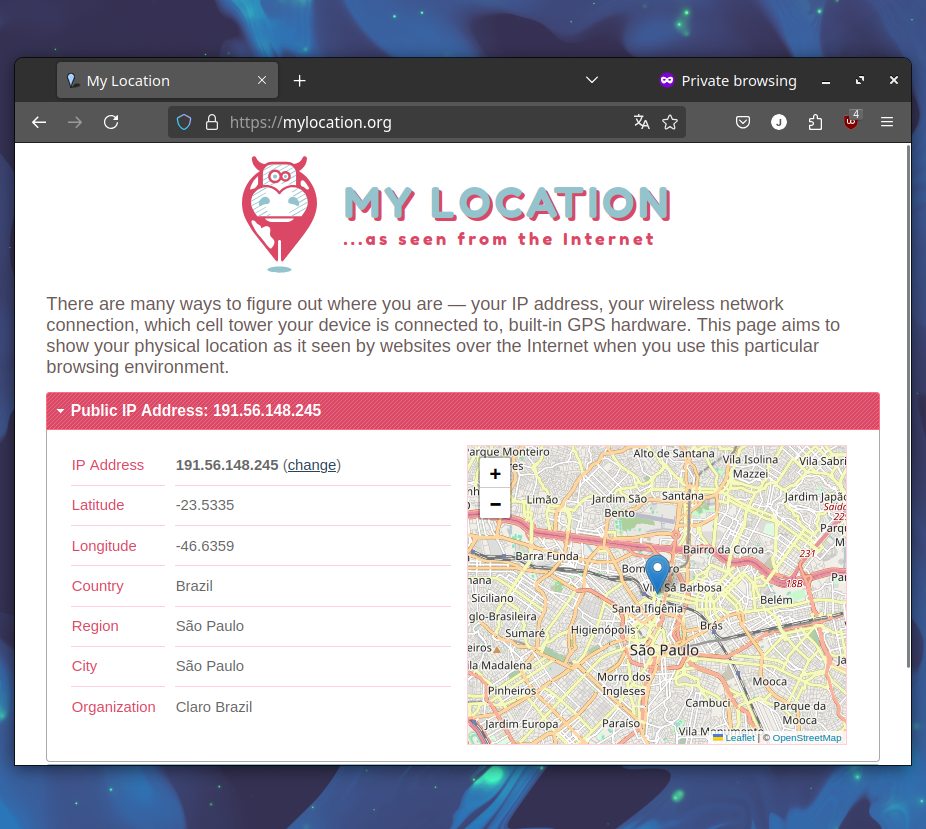
\includegraphics[width=0.85\textwidth]{loc-firefox}
    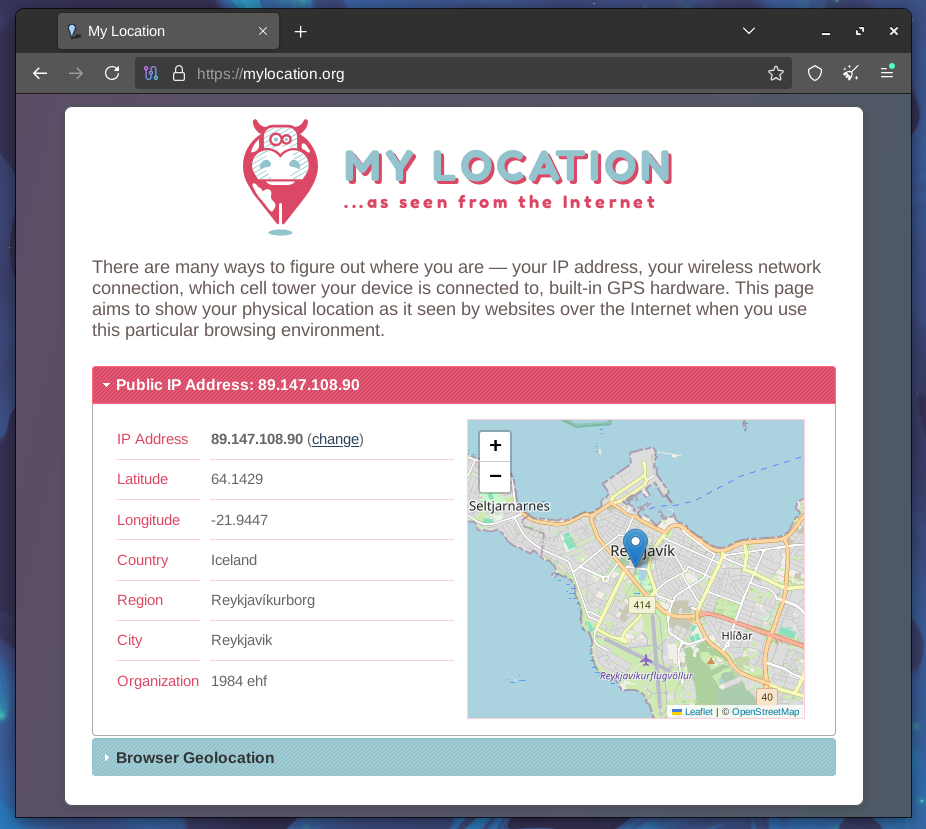
\includegraphics[width=0.85\textwidth]{loc-tor}
  
    % remember to cite the source of the image
    \caption{Captura de tela de um website de localização acessado através do \textit{Firefox} (acima) e do \textit{Tor} (abaixo). Note que mesmo usando a mesma conexão com a Internet, o website acessado através do \textit{Tor} determina a localização do \textit{Relay} de Saída (nesse caso na Islândia), e não a do usuário.}
    \label{fig:mylocation}
\end{figure}

\begin{figure}
    \centering
    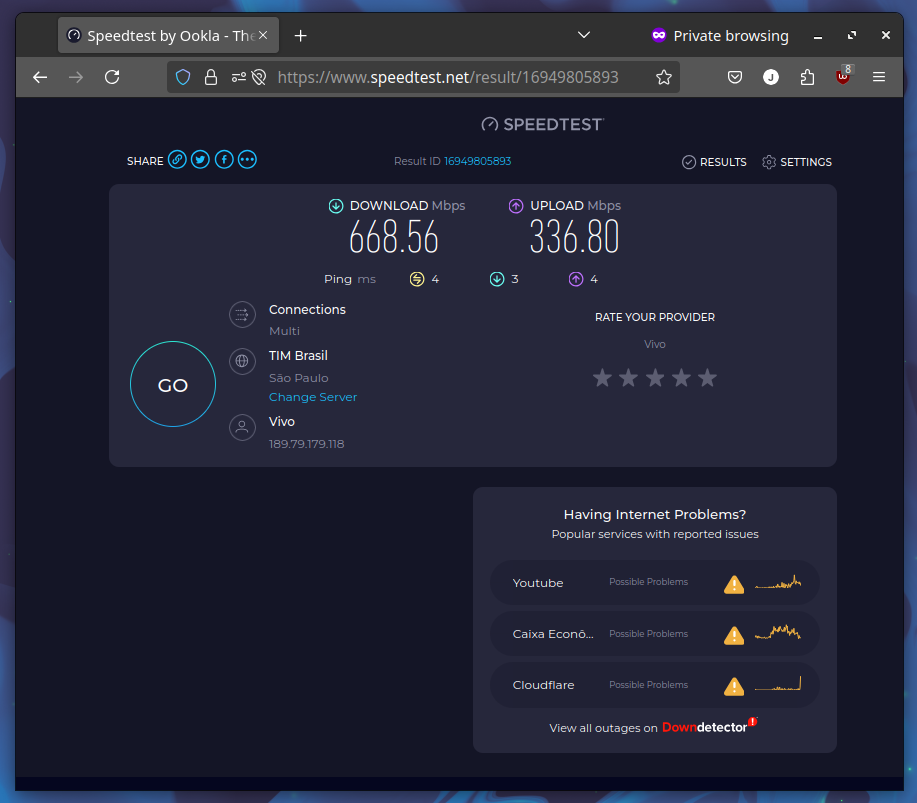
\includegraphics[width=0.85\textwidth]{speed-firefox}
    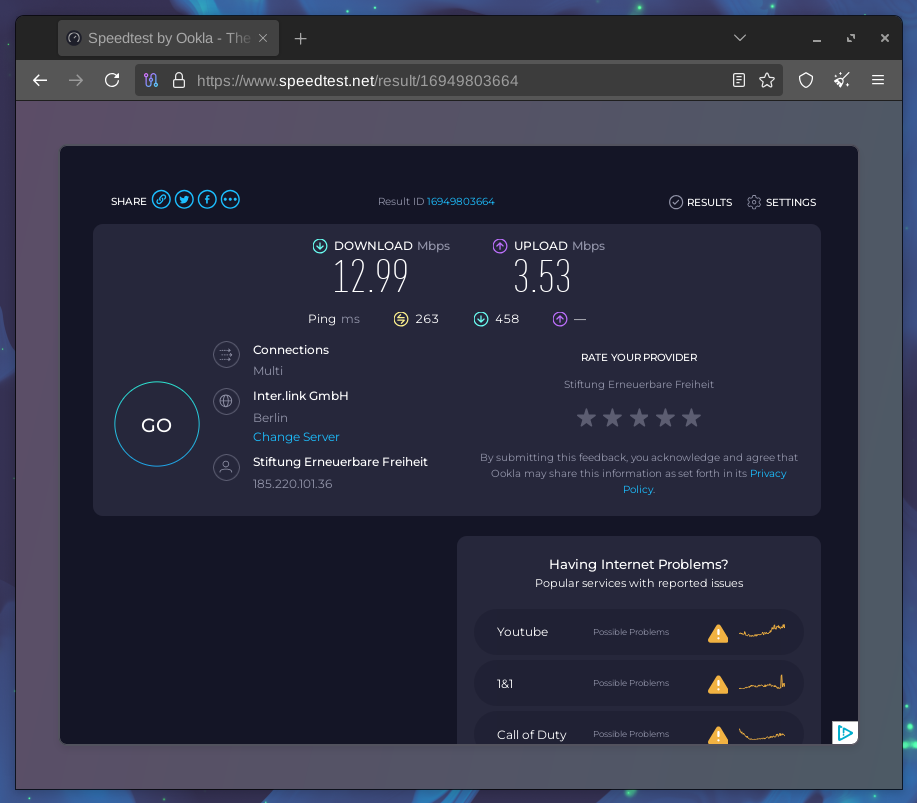
\includegraphics[width=0.85\textwidth]{speed-tor}
  
    % remember to cite the source of the image
    \caption{Captura de tela de um de teste de velocidade de conexão à Internet acessado através do \textit{Firefox} (acima) e do \textit{Tor} (abaixo). Note que a conexão através do \textit{Tor} é muito mais lenta, uma vez que o tráfego é roteado através de vários \textit{relays}, limitando a velocidade da conexão e introduzindo latência.}
    \label{fig:speedtest}
\end{figure}

Um vídeo excelente publicado pela Universidade de Nottingham que entra em mais detalhes sobre a troca de chaves e a criptografia do protocolo \textit{Tor} pode ser encontrado em \cite{computerphile-tor}.

A utilização do protocolo \textit{Tor} para acessar sites comuns da Internet é conceitualmente similar a utilizar um serviço de \textit{Virtual Private Network} (\textit{VPN}). Ambos agem como um intermediário entre o usuário e o site acessado, escondendo o endereço IP real do usuário e protegendo a sua privacidade. No entanto, enquanto \textit{Tor} é gratuito, mais anônimo e descentralizado, \textit{VPNs} são na maioria das vezes pagas e centralizadas, mas geralmente possuem melhor desempenho.

\subsection{Acesso a serviços ocultos}

Além de permitir o acesso a sites comuns da Internet de forma anônima, o \textit{Tor} também suporta a criação e acesso a serviços ocultos, que são sites que só podem ser acessados através da rede \textit{Tor}. Estes sites possuem um endereço especial, terminado em .onion, que é gerado a partir de uma chave pública do servidor. A utilização de serviços ocultos permite que os usuários hospedem sites de forma anônima e segura, contornando restrições de \textit{firewalls} e NATs, sem precisarem expor a localização física do servidor.

Quando um usuário acessa um serviço oculto, ele estabelece uma série de circuitos, buscando que tanto ele quanto o serviço oculto estabeleçam um circuito com um \textit{relay} intermediário em comum. Isso permite que o usuário e o serviço oculto possam se comunicar de forma anônima, sem que nenhum dos dois saiba a localização física do outro.

A Universidade de Nottingham também publicou um vídeo excelente que entra em mais detalhes sobre como funcionam os serviços ocultos do protocolo \textit{Tor}, que pode ser encontrado em \cite{computerphile-hidden-services}.

Uma forma de atestar o funcionamento do \textit{Tor} é por meio do acesso a algum site que verifique a geolocalização do endereço de IP do usuário, como o \textit{mylocation.org}. Esse site utiliza a base de dados de registros de IPs para informar no mínimo em qual país o usuário se encontra com base em seu endereço de IP. A figura \ref{fig:mylocation} explica como o site \textit{mylocation.org} determina a localização do \textit{relay} de saída do \textit{Tor}, e não a do usuário. Uma consequência da utlilização do \textit{Tor} é a redução na taxa de transmissão de dados e o aumento da latência nas comunicações. A figura \ref{fig:speedtest} mostra como a velocidade de conexão à Internet é reduzida quando o tráfego é roteado através de vários \textit{relays}. Ambas foram capturas de tela do mesmo website, \textit{speedtest.net}, acessado através do \textit{Firefox} e do \textit{Tor Browser}.

Serviços ocultos são extremamente úteis no contexto da transmissão segura de mensagens \textit{online}, uma vez que eles lidam com limitações de \textit{firewalls} e NATs, oferecendo comunicação que é segura e anônima. Por outro lado, a grande quantidade de intermediários no encaminhamento de mensagens significa que a latência e a velocidade da comunicação podem ser comprometidas.